	На прошлой лекции мы рассматривали задачу вариационного исчисления:
	$$I[y] = \int_{x_0}^{x_1} F(x, y, y') dx$$
	
	\opt{
	Стоит также отметить некоторые различия в терминологии. Так как задача вариационного исчисления 
	достаточно старая, дифференциал в ней принято называть \textbf{вариацией функционала}.
	}
	
	\subsection{Уравнение Эйлера}
	
	Как было замечено ранее, нашей задачей будет поиск локальных экстремумов этого функционала. В 
	курсе математического анализа необходимым условием локального экстремума было равенство нулю
	частных производных или, другими словами, равенство нулю производной по всем касательным в данной
	точке.
	
	Здесь будет использоваться подобное условие. Пусть функция $y(x)$ является экстремумом 
	рассматриваемого нашего функционала $I[y]$. Вместо касательного вектора мы рассмотрим
	функцию $h(x)$, такую, что
	$$h \in C^{\infty} \qquad \supp(h) \subset (x_0, x_1)$$
	
	\todo{Почему она будет допустимой?}
	Тогда, если $y(x)$ --- допустимая функция, то при достаточно малых $\varepsilon$, $y(x) + \varepsilon h(x)$ тоже
	будет допустимой. Введём также $J(\varepsilon) = I(y + \varepsilon h(x))$.
	
	$$J(\varepsilon) = \int_{x_0}^{x_1} F(x, y(x) + \varepsilon h(x), y'(x) + \varepsilon h'(x))\,dx$$

	Обозначим для функции $F$ её частные производные как $F_x, F_y, F_{y'}$. Возможно, стоит отметить, что частная производная
	берётся в предположении независимости переменной дифференцирования от остальных переменных функции.
	
	$$J'(\varepsilon)\lims{\varepsilon = 0}{} = \int_{x_0}^{x_1} \Big( F_{y}h(x) - F_{y'}h'(x) \Big)\,dx$$
	
	Проинтегрируем второе слагаемое в подынтегральном выражении по частям. Здесь мы делаем ранее упомянутое отклонение
	от постановки задачи: потребуется, чтобы функция $F \in C^2$, а не $C^1$.
	
	$$\int_{x_0}^{x_1} F_{y'}h'(x) \,dx = \off{F_{y'}h(x) \lims{x_0}{x_1}} - \int_{x_0}^{x_1} h(x)(\frac{d}{dx} F_y)\,dx$$
	
	$$J'(\varepsilon)\lims{\varepsilon = 0}{} = \int_{x_0}^{x_1}h(x)\cdot(F_y - \frac{d}{dx}F_{y'}) \,dx$$
	
	Из теории обобщённых функций известно, что, если регулярная обобщённая функция $f$ порождена непрерывной
	и $\forall h\:\scal{F}{h}~=~0$, то $f = 0$. Таким образом, из условия $J' = 0$ получаем \textbf{уравнение Эйлера}:
	
	\begin{equation} \label{eq:Euler}
		F_y - \frac{d}{dx}F_{y'} = 0 
	\end{equation}
	
	Равенство нулю уравнения \ref{eq:Euler} в точности совпадает с условием равенства нулю производной по всем 
	касательным векторам. Это уравнение --- необходимое условие локального экстремума функционала $I[y]$.
	
	\begin{defi}
		Функция $f(x) \in C^2$, которая является решением уравнения уравнения Эйлера, называется \textbf{экстремалью} 
		функционала $I[y]$.
	\end{defi}
	
	Рассмотрим три ситуации, когда уравнение \ref{eq:Euler} допускает понижение порядка:
	\begin{enumerate}
		\item $F(x,y,y') = F(x,y)  \Rightarrow \mathbf{F_y = 0}$
		\item $F(x,y,y') = F(x,y') \Rightarrow \mathbf{F_{y'} = C}$
		\item $F(x,y,y') = F(y,y')$. Такое уравнение возникает в задаче нахождения минимальной поверхности вращения.
		Здесь понижение порядка не столь тривиально.
		
		Рассмотрим функцию $(y'F_{y'} - F)$. Продифференцируем её по $x$:
		$$\frac{d}{dx}(y'F_{y'} - F) =
		  \off{y''F_{y'}} + y'(\frac{d}{dx}F_{y'}) - F_yy' - \off{F_{y'}y''} = 
		  y'(\frac{d}{dx}F_{y'} - F_y)$$
		
		В скобках стоит уравнение Эйлера. Тогда, если $y$ --- экстремаль, то это выражение равно нулю и уравнение 
		получается более простое:
		
		$$\mathbf{y'F_{y'} - F = C}$$
	\end{enumerate}
	
	Теперь у нас есть вся необходимая теория для решения задачи о брахистохроне --- кривой наискорейшего спуска.
	
	$$I[y] = \int_0^{x_1} \frac{\sqrt{1+y'^2}}{\sqrt{y}} \,dx$$
	
	Как видим, в данной задаче $F$ не зависит явно от $x$. Значит, выполняется случай (3).
	
	$$y'\frac{y'}{\sqrt{y(1+y'^2)}} - \frac{\sqrt{1+y'^2}}{\sqrt{y}} = C$$
	$$\frac{1}{\sqrt{y(1+y'^2)}} = C$$
	$$y(1+y'^2) = C_1$$
	Здесь и далее наиоллее частым приёмом для решения дифференциальных уравнений будет являться введение параметра.
	$$y' = ctg(v)$$
	$$y = C_1 \sin^2(v) = \frac{C_1}{2}(1 - \cos(2v))$$
	Осталось найти $x = x(v)$ и решение будет получено.
	
	$$\frac{dx}{dv} = \frac{dy}{dv} \frac{1}{y'} = 
	  \frac{C_1\sin(2v)}{ctg(v)} = \frac{2C_1 \sin^2(v)\cos(v)}{\cos(v)} = C_1\big(1 - cos(2v)\big)$$
	  
	Интегрируя данное уравнение по $v$, получаем $x(v)$:
	$$x(v) = C_1\left(v - \frac{\sin(2v)}{2}\right) + C_2$$
	
	Получаем параметризованное решение уравнения:
	
	\begin{align*}
		x = \frac{C_1}{2} \big(t - \sin(t)\big) + C_2 \\
		y = \frac{C_1}{2} \big(1 - \cos(t)\big)
	\end{align*}
	
	Из начальных условий, при $t = 0$, $x = 0$. Таким образом $C_2 = 0$.

	\begin{figure}[H]
		\begin{subfigure}[c]{0.5\textwidth}
		\begin{align*}
			x = C \big(t - \sin(t)\big) \\
			y = C \big(1 - \cos(t)\big)
		\end{align*}	
		\end{subfigure}
		~
		\begin{subfigure}[c]{0.5\textwidth}
			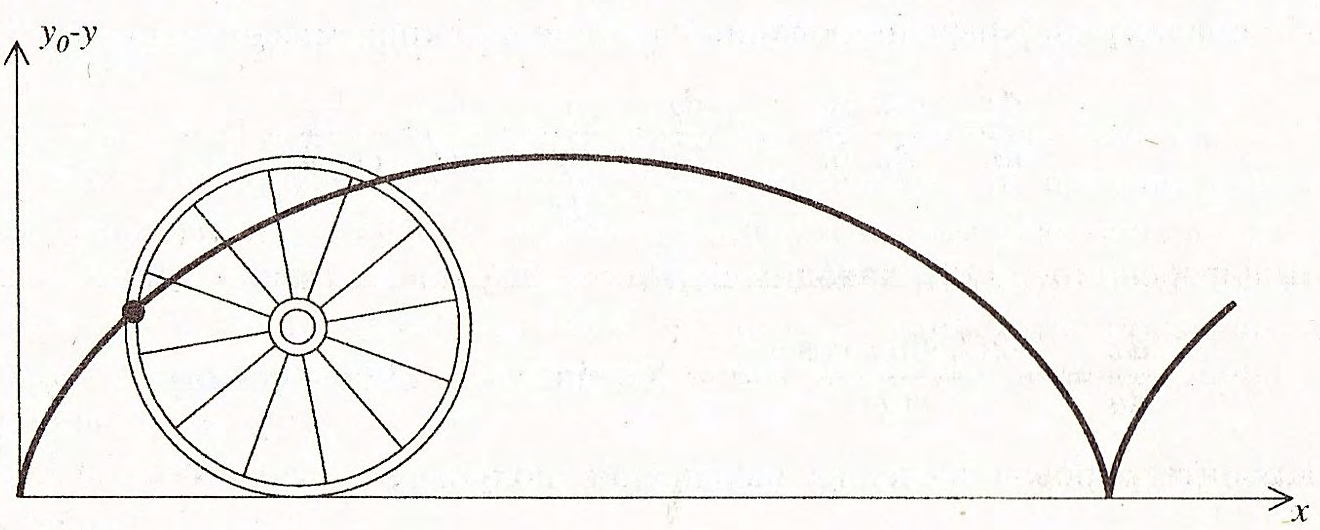
\includegraphics[width=0.8\textwidth]{../Graphics/Lectures-12-cycloid.png}
			\caption{\footnotesize Циклоида \copyvar{С. 22.}}
		\end{subfigure}
	\end{figure}
	
	Следовательно, кривая наименьшего спуска является циклоидой.
	
	Для решения задач вариационного исчисления может потребоваться большее число функций или независимых переменных.
	К примеру, задача нахождения геодезической кривой, в которой требуется найти $x(t), y(t), z(t)$, которые определяют
	кратчайший путь между двумя точками на поверхности трёхмерной фигуры.
	
	Итак, если есть несколько функций $y$:
	$$F = F(x, y_1, y_1', y_2, y_2',\ldots)$$
	
	Тогда просто записывается система уравнений Эйлера:
	$$\left\{
	  \begin{aligned}
	  	  F_{y_1} - \frac{d}{dx}F_{y_1'} = 0 \\
	  	  \dots\\
	  	  F_{y_n} - \frac{d}{dx}F_{y_n'} = 0
	  \end{aligned}
	  \right.$$
	
	Рассмотрим случай, когда появляются производные более высоких порядков. 
	$$F = F(x, y, y', \ldots, y^{(k)})$$	
	Как и раньше, введём $J(\varepsilon) = I[y + \varepsilon h]$. $J'(\varepsilon)$ запишется следующим образом:
	
	$$J'(\varepsilon)\lims{\varepsilon = 0}{} = \int_{x_0}^{x_1} (F_y h(x) + F_{y'}h'(x) 
	  + F_{y''}h''(x) + \ldots + F_{y^{(k)}}h^{(k)})\,dx$$
	
	Первое слагаемое ранее уже интегрировали по частям: 
	$$\int_{x_0}^{x_1} F_{y'}h'(x)\,dx~=~-~\int_{x_0}^{x_1} h(x)\left(\frac{d}{dx} F_{y'}\right)\,dx$$
	Рассмотрим таким же образом следующее слагаемое:
	
	$$\int_{x_0}^{x_1} F_{y''}h'' \,dx = \off{h'(x)F_{y''}\lims{x_0}{x_1}} - \int_{x_0}^{x_1} h'(x)\frac{d}{dx}F_{y''} \,dx
	  = \off{-h(x)\frac{d}{dx} F_{y''}\lims{x_0}{x_1}} + \int_{x_0}^{x_1} h(x) \frac{d^2}{dx^2}F_{y''} \,dx$$
	  
	Как и ранее, выделенные серым слагаемые равняются нулю из-за того, что
	функции $h^{(k)}(x)$ равны нулю на краях отрезка $[x_0, x_1]$.
	
	Преобразовав все слагаемые таким образом, перепишем $J'(\varepsilon)$:
	$$\int_{x_0}^{x_1} h(x)
	  \underbrace{\left(F_y - \frac{d}{dx}F_{y'} + \frac{d^2}{dx^2}F_{y''} - 
	  \ldots + (-1)^k\frac{d^k}{dx^k}F_{y^{(k)}}\right)}_{f(x, y, \ldots, y^{(k)})} \,dx$$
	
	Так же как и раньше, необходимым условием будет являться выполнение уравнения $f = 0$.
	
	\begin{equation} \label{eq:EulerPoisson}
		F_y - \frac{d}{dx}F_{y'} + \frac{d^2}{dx^2}F_{y''} - 
	  \ldots + (-1)^k\frac{d^k}{dx^k}F_{y^{(k)}} = 0
	\end{equation}
	
	Уравнение \ref{eq:EulerPoisson} называется \textbf{уравнением Эйлера-Пуассона}.
	
	Осталось рассмотреть ситуацию, когда возникает несколько независимых переменных. Тогда рассмотрим функцию
	$z = z(x,y)$ и функционал
	$$I[z] = \underset{D\hspace{10pt}}{\iint} F(x, y, z, z'_x, z'_y) \,dxdy$$
	
	Здесь мы снова введём $h \in C^{\infty}$, $\supp(h) \subset D$, $D$ --- открытая область. Также введём
	$J(\varepsilon) = I[z + \varepsilon h]$. Тогда 
	$$J'(\varepsilon)\lims{\varepsilon = 0}{} = 
	  \underset{D\hspace{10pt}}{\iint} (F_zh + \underline{F_{z'_x}h'_x} + \underline{F_{z'_y}h'_y}) \,dxdy$$
	  
	Чтобы получить уравнение на экстремали, нужно получить $h(x)$ вместо её производных в подчёркнутых слагаемых.
	
	\begin{align*}
		\frac{d}{dx}(h F_{z'_x}) = \underline{h'_xF_{z'_x}} + h\frac{d}{dx}F_{z'_x} \\
		\frac{d}{dy}(h F_{z'_y}) = \underline{h'_yF_{z'_y}} + h\frac{d}{dy}F_{z'_y}
	\end{align*}
	
	Перепишем $J(\varepsilon)$, выразив подчёркнутые слагаемые.
	
	$$
		J'(\varepsilon)\lims{\varepsilon = 0}{} = 
		\underset{D\hspace{10pt}}{\iint} \left( h\cdot\left(F_z - \frac{d}{dy}F_{z'_y} - \frac{d}{dx}F_{z'_x}\right) \right) \,dxdy
		+ \underset{D\hspace{10pt}}{\iint} \left(\frac{d}{dx}(hF_{z'_x}) + \frac{d}{dy}(hF_{z'_y}) \right) \,dxdy
	$$
	Второй интеграл может быть преобразован по теореме Стокса. В двумерном случае 
	$\iint_{D} (P\,dx + Q\,dy) = \oint_{\partial D} (Q_x - P_y) dx dy$.
	$$
		J'(\varepsilon)\lims{\varepsilon = 0}{} = 
		\underset{D\hspace{10pt}}{\iint} \left( h\cdot\left(F_z - \frac{d}{dy}F_{z'_y} - \frac{d}{dx}F_{z'_x}\right) \right) \,dxdy
		+ \underbracket{\underset{\partial D}{\oint} \left(hF_{z'_x}\,dy + hF_{z'_y}\,dx \right)}_{=0}
	$$
	
	Второй интеграл равняется нулю, так как функция $h(x, y)\lims{\partial D}{} \equiv 0$ потому что $\supp(h) \subset D$.
	
	Полученное уравнение 
	$$F_z - \frac{d}{dy}F_{z'_y} - \frac{d}{dx}F_{z'_x} = 0$$
	называется \textbf{уравнением Эйлера-Остроградского}.
	
	$$I[y] = \int_{x_0}^{x_1} F(x, y, y')dx \qquad y(x_0) = y_0$$
	
	\begin{figure}
		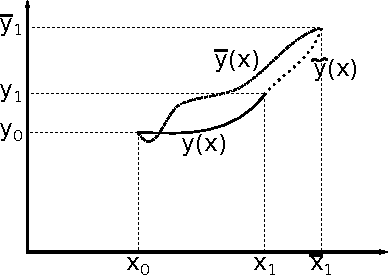
\includegraphics[width=0.8\textwidth]{./../Graphics/Lectures-12-unknowntask.pdf}
	\end{figure}
	
	Продолжим функцию $y(x)$ так, чтобы её продолжение
	$\tilde{y}(x) \in C^1$.
	
	Введём $\rho(y, \tilde{y}) = 
	\norm{y - \tilde{y}} + \sqrt{(x_1 - \bar{x_1})^2 + (y_1 - \bar{y_1})^2}$
	
	Назовём $\rho$ расстоянием между двумя этими функциями.
	
	Для дальнейших вычислений введём следующие обозначения:
	
	$$
		\left\{
		\begin{aligned}
			h(x) = \overline{y} - y \\
			\delta x = \overline{x_1} - x_1
		\end{aligned}
		\right.
	$$
	
	$$I[\overline{y}] - I[y] = 
	  \underbracket{\int_{x_0}^{x_1} (F(x, y + h, y' + h') - F(x, y, y')) \,dx}_{I_1} +
	  \underbracket{\int_{\overline{x}_0}^{\overline{x}_1} F(x, \overline{y}, \overline{y}') \,dx}_{I_2}$$
	  
	В подынтегральном выражении для $I_2$ стоит непрерывная функция. Значит, можем воспользоваться теоремой о среднем.
	
	\opt{
		\begin{theorem*}
			Пусть функция f(x) непрерывна на $[x_1, \overline{x}_1]$, тогда 
			$\exists x_C\in[x_1,\overline{x}_1]\;\;
			\int\limits_{x_1}^{\overline{x}_1}f(x)dx = f(x_C)(\overline{x}_1 - x_1)$.
		\end{theorem*}
	}
	
	Положим некоторое значение $x_C \in [x_0, x_1]$. Тогда 
	$$I_2 = \delta x_1 F(x, \overline{y}, \overline{y}')\lims{x = x_C}{} 
	= \delta x_1 F\big(x_1, \overline{y}(x_1), \overline{y}'(x_1)\big) + o(\delta x_1)$$
	
	Приращение интеграла $I_1$ можно записать по формуле Тейлора:
	$$f(x + h) = f(x) + df(x) \angular{h} + o(\mod{h})$$
	Таким образом, 
	$$I_1 = \int_{x_0}{x_1} (F_yh - F_{y'}h') \,dx + o\big(\rho(y, \overline{y})\big)$$
	
	$o(\ldots)$ ушло из подынтегрального выражения, так как интеграл берётся по конечному промежутку, а 
	умножение $o(\ldots)$ на константу ничего не меняет. Итак, интегрируем второго слагаемое по частям.
	
	$$I_1 = \int_{x_0}{x_1} h\cdot(F_y - \frac{d}{dx}F_{y'}) \,dx + hF_{y'}\lims{x_0}{x_1} + o(\ldots) = 
	  \int_{x_0}^{x_1} h\cdot(F_y - \frac{d}{dx}F_{y'}) \,dx + h(x_1) F_{y'}\lims{x = x_1}{}$$
	  
	\off{Дописать не успели, закончилась лекция.}
	
	\textbf{Интеграл Дирихле}. Рассмотрим функционал вида 
	
	$$I[z] = \iint\limits_D (z_x'^2 + z_y'^2)^2 \,dxdy$$
	
	Рассматриваемый интеграл называется интегралом Дирихле. Получим выражение 
	для экстремалей функционала $I[z]$.
	
	$$\off{F_z} - \frac{d}{dy} F_{z'_y} - \frac{d}{dx} F_{z'_x} = 0$$
	$$-\frac{d}{dy} 2z'_y - \frac{d}{dx} 2z'_x = 0$$
	$$z''_{yy} + z''_{xx} = 0$$
	
	Таким образом, экстремалями этого функционала являются гармонические функции.